\documentclass[aps,prb,reprint,nofootinbib]{revtex4-2}

\usepackage{amsmath,amssymb}
\usepackage{graphicx}
\usepackage{booktabs}
\usepackage{listings}
\usepackage{xcolor}

\definecolor{codekw}{HTML}{0072B2}
\definecolor{codestr}{HTML}{009E73}
\definecolor{codecom}{HTML}{777777}

\lstset{
  language=Python,
  basicstyle=\ttfamily\scriptsize,
  keywordstyle=\color{codekw},
  stringstyle=\color{codestr},
  commentstyle=\color{codecom}\itshape,
  numbers=left, numberstyle=\tiny\color{codecom}, numbersep=7pt,
  frame=single, rulecolor=\color{codecom},
  breaklines=true, breakatwhitespace=true,
  showstringspaces=false, tabsize=4,
  columns=fullflexible, keepspaces=true,
  extendedchars=true, inputencoding=utf8,
  literate=%
    {ω}{{$\omega$}}1 {π}{{$\pi$}}1 {μ}{{$\mu$}}1 {η}{{$\eta$}}1
    {→}{{$\rightarrow$}}1 {≤}{{$\le$}}1 {≥}{{$\ge$}}1
    {—}{{---}}1 {–}{{--}}1 {×}{{$\times$}}1 {⁻}{{$^-$}}1 {¹}{{$^1$}}1
    {⁵}{{$^5$}}1 {−}{{$-$}}1
}

\usepackage{hyperref}
\hypersetup{colorlinks=true, linkcolor=black, citecolor=black,
            filecolor=black, urlcolor=blue}

\graphicspath{{../figures/}}

\begin{document}

\title{Fermi--Dirac Statistics in a Semiconductor Crystal%
\thanks{Solid State Physics, Assignment 1 --- Question 5.}}

\author{Guhan Dhanasekharan\,\,(EP24BTECH11011)}
\author{Kumud Jalori\,\,(EP24BTECH11015)}
\author{Naman Verma\,\,(EP24BTECH11016)}
\author{Nazakar Abhilash\,\,(EP24BTECH11017)}
\author{Nithin Surya S\,\,(EP24BTECH11018)}
\author{Panduru Sri Abish\,\,(EP24BTECH11019)}
\author{Prasang Das\,\,(EP24BTECH11020)}
\author{Praveen Kumar\,\,(EP24BTECH11021)}
\author{S Haresh\,\,(EP24BTECH11022)}
\author{S Kshiteesh\,\,(EP24BTECH11023)}
\affiliation{Department of Engineering Physics}

\date{\today}

\begin{abstract}
We compute the electronic occupation statistics of a parabolic-band semiconductor by solving the
carrier-density integral $n=\int D(E)f(E)\,dE$ numerically for the chemical potential. Writing
the integral in terms of the dimensionless Fermi--Dirac integral $F_{1/2}$ keeps the units in one
place and makes the integration cutoff a multiple of $k_BT$. The implementation is validated
against both analytic limits: it reproduces the non-degenerate Boltzmann result to
$1.3\times10^{-4}$ and the degenerate $T\to0$ Fermi energy to $10^{-7}$, and its temperature
dependence follows the Sommerfeld expansion to $4\times10^{-9}$. An interactive Streamlit
interface exposes temperature, carrier concentration, effective mass and band gap, and reports
$E_F$, $k_F$, $v_F$ and $T_F$ alongside a degeneracy flag. We stress a distinction the usual
phrasing obscures: the quantity that varies with temperature is the chemical potential
$\mu(T)$, not the Fermi energy $E_F=\mu(0)$, and $k_F$, $v_F$ and $T_F$ are meaningful only
when the carrier gas is degenerate --- which at room temperature requires
$n \gtrsim 10^{18}\,$cm$^{-3}$.
\end{abstract}

\maketitle

\section{Introduction}

The electrons in a crystal are indistinguishable spin-$\tfrac12$ fermions, so the Pauli principle
limits each state to one of them. Their equilibrium distribution over energy is therefore not
the Boltzmann distribution of classical statistics but the Fermi--Dirac distribution. In a metal
this distinction is dramatic: the electron gas is degenerate, the occupation is essentially a
step, and only electrons within $k_BT$ of the Fermi level participate in transport or heat
capacity. In a lightly doped semiconductor the carriers are dilute enough that Fermi--Dirac
statistics reduce to Boltzmann statistics and the distinction nearly vanishes.

A semiconductor is interesting precisely because it can be moved between these two regimes by
doping. This report computes where the boundary lies, by solving for the chemical potential
without approximating the statistics, and uses that to examine how the Fermi level moves with
temperature and carrier concentration.

\section{Theory}
\label{sec:theory}

\subsection{Fermi--Dirac statistics}

The mean occupation of a single-particle state of energy $E$ in equilibrium at temperature $T$ is
\begin{equation}
  f(E) = \frac{1}{\exp\!\big((E-\mu)/k_BT\big)+1},
  \label{eq:fd}
\end{equation}
where $\mu$ is the chemical potential. Two properties follow immediately and are used
throughout. First, $f(\mu)=\tfrac12$ at every temperature, so $\mu$ is the energy at which a
state is equally likely to be occupied or empty. Second, as $T\to0$, $f$ becomes a step: every
state below $\mu$ is filled, every state above is empty.

\subsection{Density of states}

In a cubic box of side $L$ with periodic boundary conditions the allowed wavevectors form a
lattice of spacing $2\pi/L$, so $k$-space contains $(L/2\pi)^3$ states per unit volume, doubled
for spin. Counting states in a shell of radius $k$ and converting to energy with the
effective-mass dispersion $E = E_c + \hbar^2k^2/2m^*$ gives the conduction-band density of
states per unit volume,
\begin{equation}
  D(E) = \frac{1}{2\pi^2}\left(\frac{2m^*}{\hbar^2}\right)^{3/2}\sqrt{E-E_c},
  \qquad E \ge E_c,
  \label{eq:dos}
\end{equation}
and zero inside the gap. The square-root edge is the three-dimensional signature: states become
available gradually above the band edge rather than all at once.
Figure~\ref{fig:kspace} sets out the counting.

\begin{figure}[t]
\centering
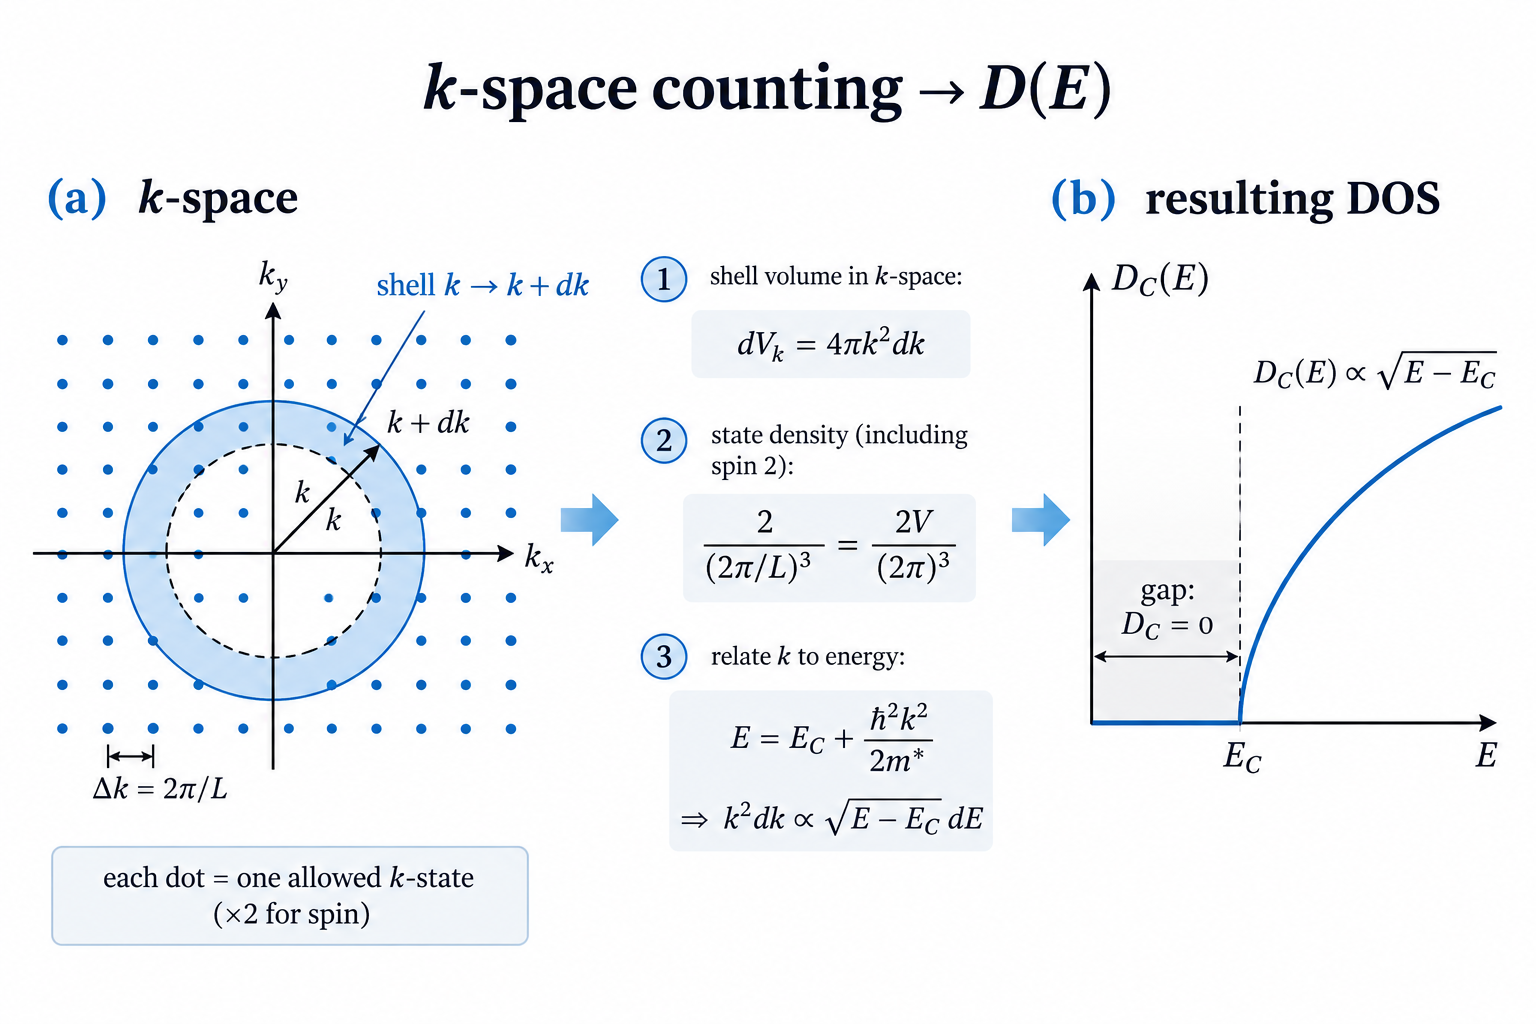
\includegraphics[width=\columnwidth]{kspace_dos.png}
\caption{Counting states in $k$-space to obtain $D(E)$. (a) Periodic boundary conditions put the
allowed wavevectors on a lattice of spacing $\Delta k = 2\pi/L$; the sketch is a section through
the three-dimensional grid, while the shell volume $4\pi k^2 dk$ in step 1 is the full
three-dimensional one. Dividing that shell volume by the volume per state and doubling for spin
gives the number of states it holds; step 3 converts $dk$ to $dE$ through the effective-mass
dispersion. Carrying the constants through gives
$D(E)=(1/2\pi^{2})(2m^{*}/\hbar^{2})^{3/2}\sqrt{E-E_{c}}$ per unit volume, the result quoted as
Eq.~\eqref{eq:dos}. (b) The resulting band-edge behaviour, written $D_C(E)$ in the figure and
$D(E)$ in the text: identically zero below $E_c$, rising with a vertical tangent at the edge and
as $\sqrt{E-E_c}$ above it. Every later figure in this report inherits that square-root shape.}
\label{fig:kspace}
\end{figure}

\subsection{Carrier density fixes the chemical potential}

The carrier concentration is the occupied density of states, integrated:
\begin{equation}
  n = \int_{E_c}^{\infty} D(E)\,f(E)\,dE.
  \label{eq:n}
\end{equation}
Given $n$, $T$ and $m^*$, this is one equation in the single unknown $\mu$. Substituting
$x=(E-E_c)/k_BT$ and $\eta=(\mu-E_c)/k_BT$ reduces it to a dimensionless form,
\begin{equation}
  n = N_c\,\frac{2}{\sqrt{\pi}}\,F_{1/2}(\eta),
  \qquad
  F_{1/2}(\eta)=\int_0^\infty\!\frac{\sqrt{x}\,dx}{1+e^{\,x-\eta}},
  \label{eq:fermiint}
\end{equation}
with the effective conduction-band density of states
$N_c = 2\left(m^*k_BT/2\pi\hbar^2\right)^{3/2}$. This is the form we solve: it isolates all
dimensional factors in $N_c$ and makes the integration cutoff a multiple of $k_BT$ rather than a
fixed energy, which matters because the degenerate case extends far above the band edge.

\subsection{The two limits}

\paragraph{Non-degenerate ($\eta \ll -1$).} The $+1$ in the denominator of \eqref{eq:fd} is
negligible, $F_{1/2}(\eta)\to(\sqrt\pi/2)e^\eta$, and \eqref{eq:fermiint} collapses to the
Boltzmann result
\begin{equation}
  n = N_c\exp\!\left(\frac{\mu-E_c}{k_BT}\right).
  \label{eq:boltz}
\end{equation}
The chemical potential lies \emph{below} the band edge, there is no Fermi surface, and the
carriers behave as a classical gas.

\paragraph{Degenerate ($\eta \gg 1$).} Here $F_{1/2}(\eta)\to\tfrac23\eta^{3/2}$ and
\eqref{eq:fermiint} inverts to
\begin{equation}
  E_F \equiv \mu(T{=}0) - E_c = \frac{\hbar^2}{2m^*}\left(3\pi^2 n\right)^{2/3},
  \label{eq:EF}
\end{equation}
the familiar free-electron-gas result. The corresponding Fermi wavevector, velocity and
temperature are
\begin{equation}
  k_F = (3\pi^2n)^{1/3},\quad v_F = \frac{\hbar k_F}{m^*},\quad T_F = \frac{E_F}{k_B}.
  \label{eq:kf}
\end{equation}

\subsection{Two points of care}

\paragraph{$E_F$ is not $\mu(T)$.} The two coincide only at $T=0$. Equation~\eqref{eq:EF}
defines $E_F$ as a function of $n$ alone, with no temperature in it; the quantity that moves
when the temperature changes is $\mu(T)$, obtained from \eqref{eq:fermiint}. Where this report
plots a ``Fermi level versus temperature'' it plots $\mu(T)$, and the distinction is not
cosmetic: in Fig.~\ref{fig:muT}(a) the $n=10^{16}\,$cm$^{-3}$ curve falls by $0.3$ eV over the
range shown while its $E_F$ is fixed at $2.5$ meV.

\paragraph{$k_F$, $v_F$ and $T_F$ presuppose degeneracy.} They describe a filled Fermi sphere.
For $n=10^{16}\,$cm$^{-3}$ in GaAs, Eq.~\eqref{eq:kf} returns $T_F = 29$ K --- far below room
temperature, which is precisely the statement that the gas is \emph{not} degenerate at $300$ K
and that these quantities are formal numbers rather than physical ones. The interface therefore
reports them as asked and displays $\eta$ beside them so the regime is never in doubt.

\section{Numerical method}

\begin{enumerate}
  \item Evaluate $F_{1/2}(\eta)$ by quadrature, with the upper limit at $\max(\eta,0)+60$;
        the integrand falls off as $e^{-(x-\eta)}$, so this is far past negligible.
  \item Solve $n(\eta)=n_{\text{target}}$ for $\eta$ with Brent's method.
  \item Bracket by widening geometrically until the residual changes sign. A fixed bracket
        fails at low temperature, where $n(\eta)$ is nearly a step.
  \item Return $\mu = E_c + \eta k_BT$.
\end{enumerate}
Evaluating $f(E)$ through the logistic function \texttt{expit} avoids overflow when
$|E-\mu|\gg k_BT$, which otherwise produces \texttt{inf} and a silent \texttt{nan}.

\subsection{Validation}

Six checks run in \texttt{test\_fermi.py}; all pass.

\begin{table}[h]
\centering
\small
\begin{tabular}{lr}
\toprule
\textbf{Check} & \textbf{Result} \\
\midrule
Non-degenerate limit vs Eq.~\eqref{eq:boltz}      & $1.3\times10^{-4}$ \\
Degenerate $T\to0$ limit vs Eq.~\eqref{eq:EF}     & $9.6\times10^{-8}$ \\
Carrier-density round trip                        & $4.9\times10^{-14}$ \\
$f(\mu)=\tfrac12$                                 & exact \\
Sommerfeld expansion for $\mu(T)$                 & $3.6\times10^{-9}$ \\
$D(E)$ zero in the gap, analytic above $E_c$      & exact \\
\bottomrule
\end{tabular}
\caption{Validation results, as maximum relative errors.}
\label{tab:valid}
\end{table}

The fifth is the strongest: in the degenerate regime the Sommerfeld expansion predicts
\begin{equation}
  \mu(T) \simeq E_F\left[1-\frac{\pi^2}{12}\left(\frac{k_BT}{E_F}\right)^{2}\right],
  \label{eq:somm}
\end{equation}
and the numerical solution follows this $T^2$ law to nine digits, as
Fig.~\ref{fig:muT}(b) shows. That tests the temperature dependence quantitatively rather than
merely checking its sign.

\section{The interactive interface}

The interface is written with Streamlit and launched with \texttt{streamlit run app.py}. The
sidebar takes the band gap, effective mass, temperature, carrier concentration and energy range,
with presets for GaAs, Si and Ge. The main panel reports $\mu-E_c$, $E_F$, $k_F$, $v_F$ and
$T_F$, states which regime the parameters fall in, and plots the band edges with $f(E)$ on a
shared energy axis, $D(E)$ with its occupied part, and both sweeps. Every change recomputes the
full integral; nothing is approximated for speed.

\begin{figure*}[t]
\centering
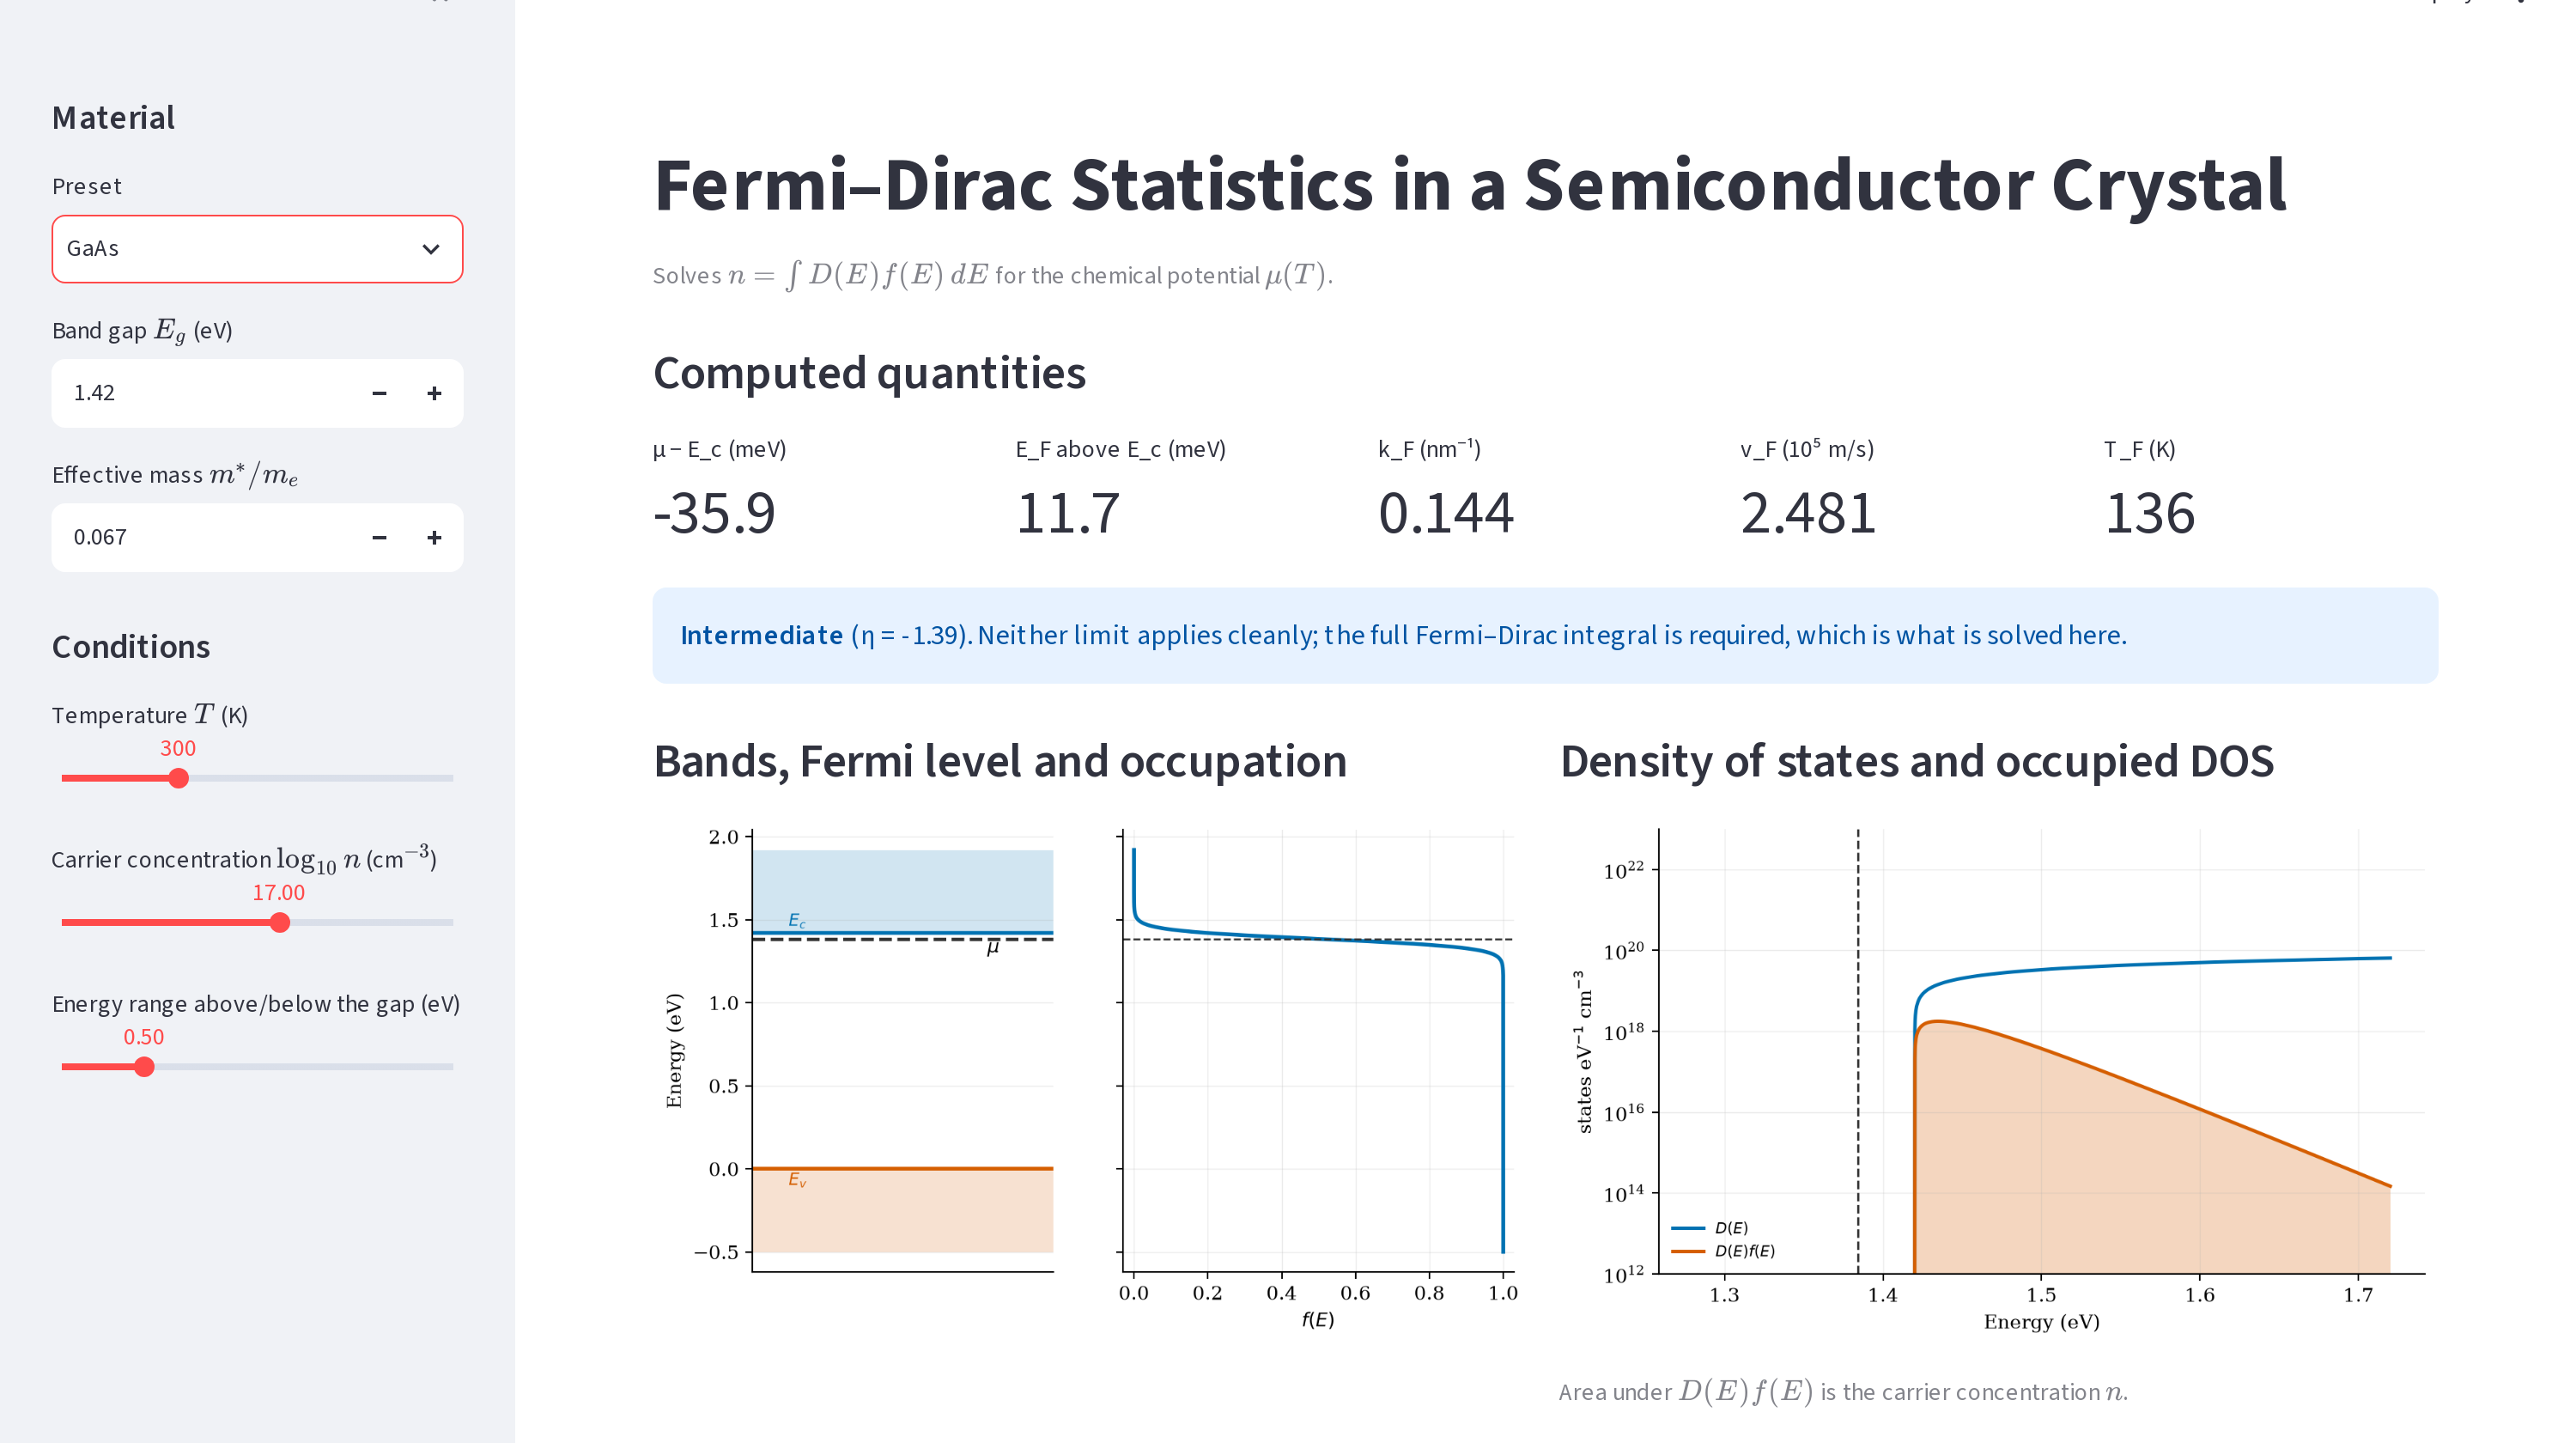
\includegraphics[width=0.92\textwidth]{ui_gaas_top.png}
\caption{The interface on the GaAs preset at $T=300$ K and $n=10^{17}\,$cm$^{-3}$. The banner
reports $\eta=-1.39$: neither limit applies cleanly here, which is why the full integral is
solved rather than either closed form.}
\label{fig:ui}
\end{figure*}

\section{Results}

Unless stated otherwise the material is GaAs-like, $E_g=1.42$ eV and $m^*=0.067\,m_e$, at
$T=300$ K.

\begin{figure}[t]
\centering
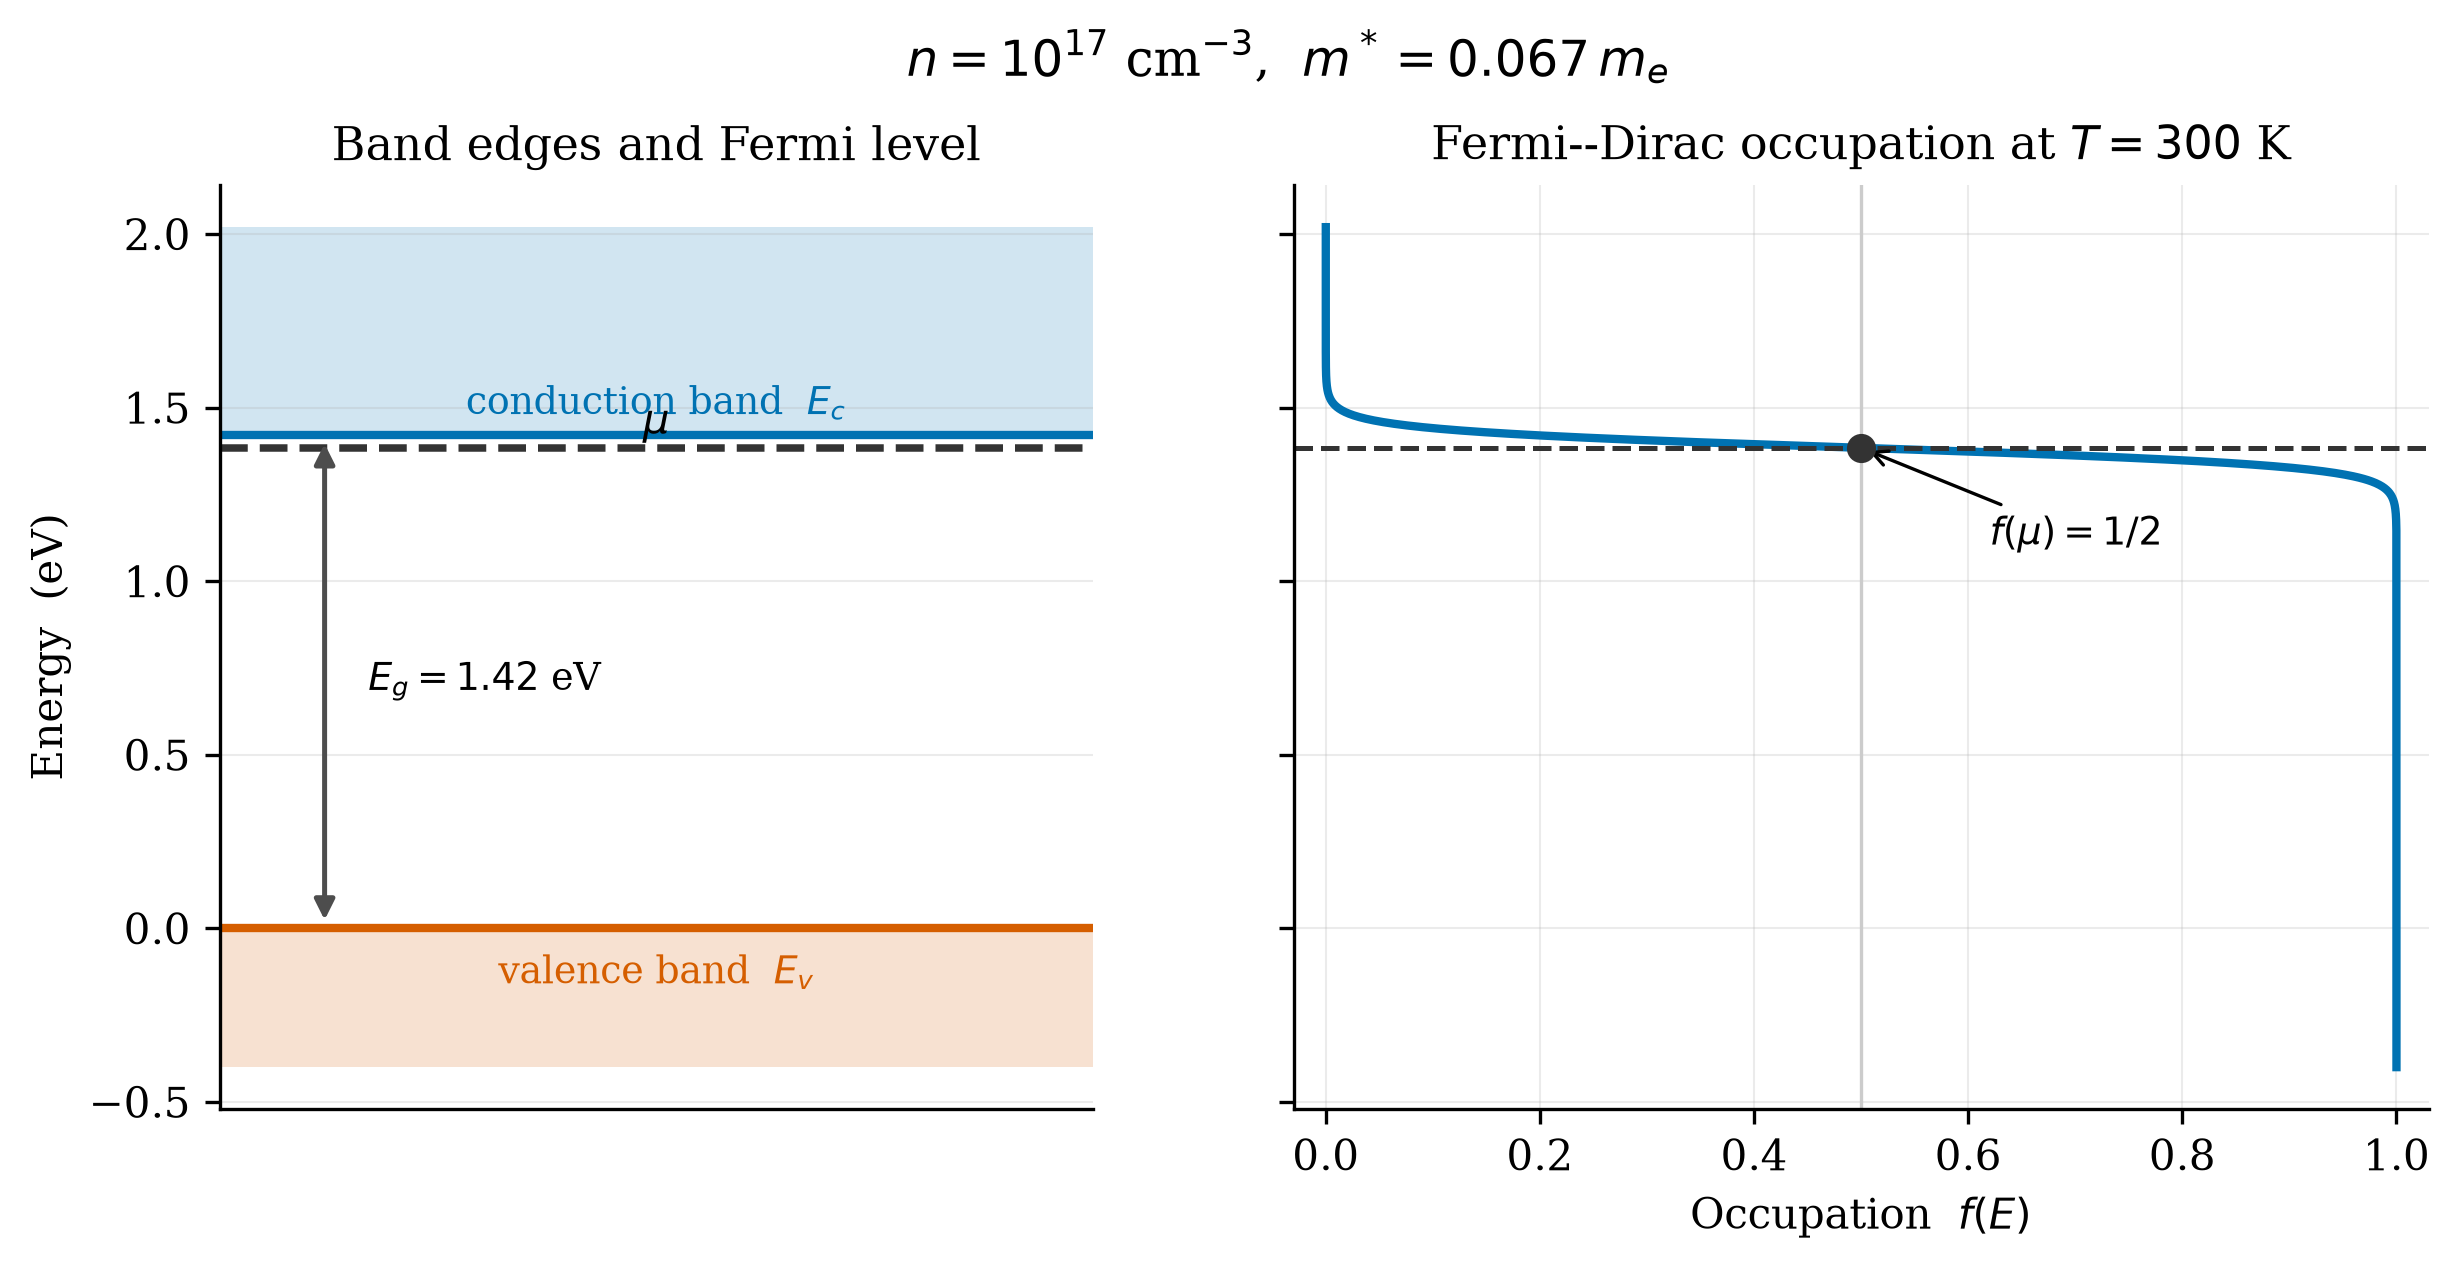
\includegraphics[width=\columnwidth]{bands.png}
\caption{Band edges, chemical potential and the Fermi--Dirac occupation on a shared energy axis,
at $n=10^{17}\,$cm$^{-3}$. $f(E)$ passes through $\tfrac12$ exactly at $\mu$.}
\label{fig:bands}
\end{figure}

\begin{figure}[t]
\centering
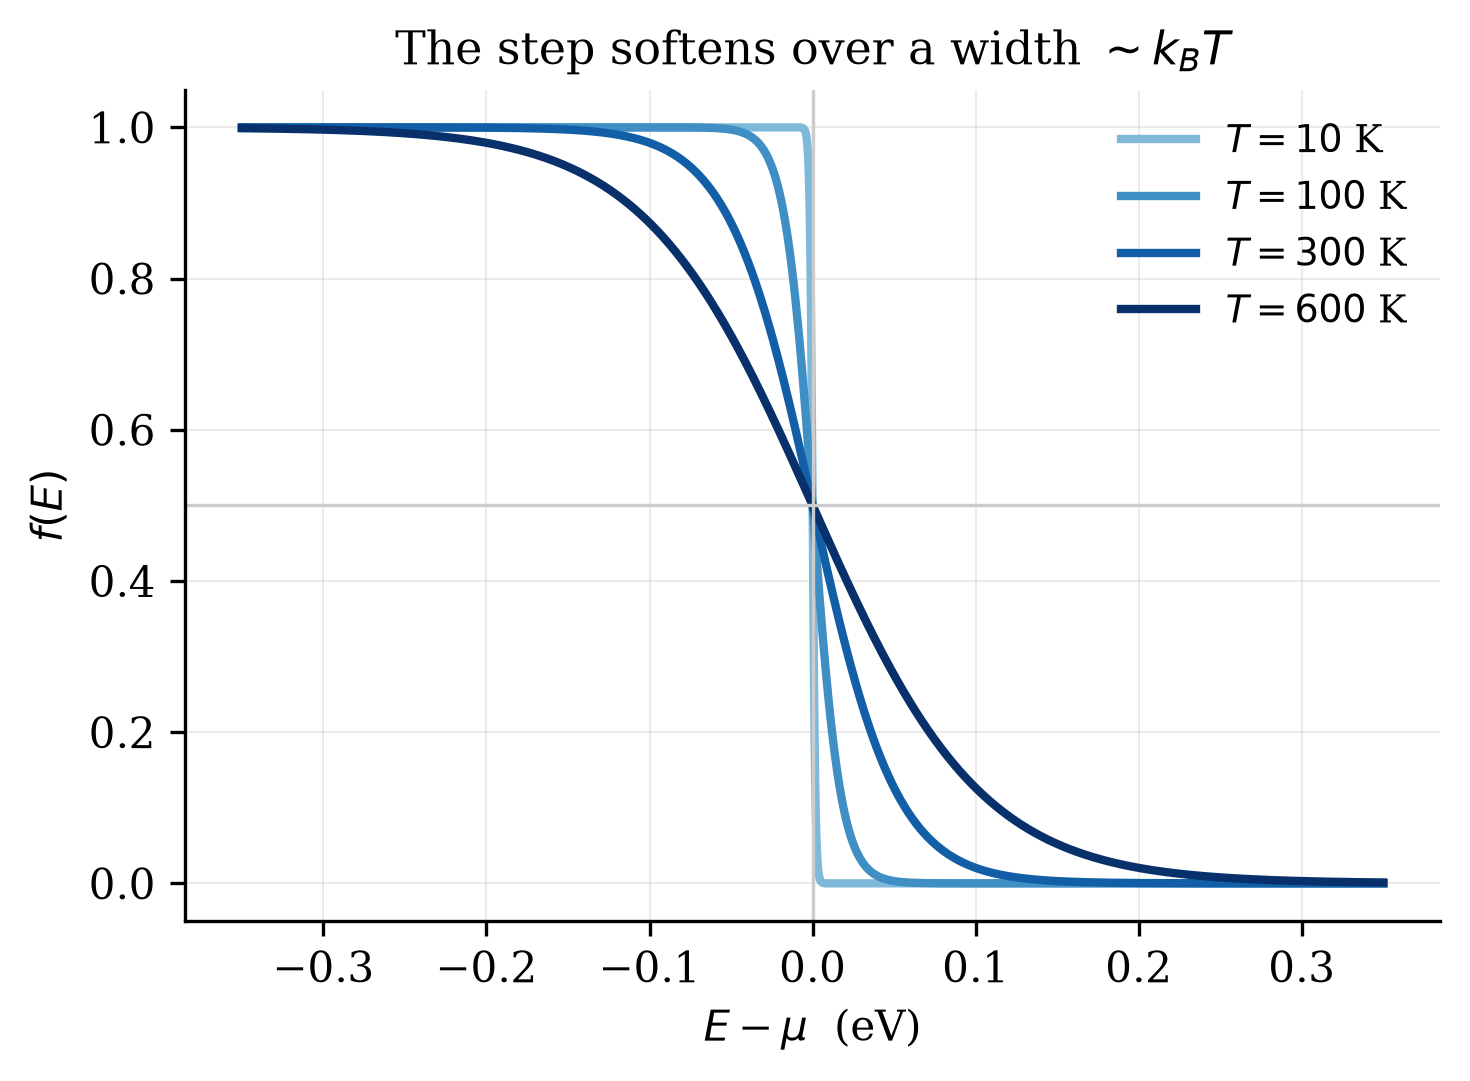
\includegraphics[width=\columnwidth]{occupation.png}
\caption{The occupation step softens over a width of order $k_BT$. At $10$ K it is nearly the
$T=0$ step; at $600$ K it is smeared over more than $0.2$ eV. The curves share a single reference
$\mu$, solved at $300$ K and $10^{19}\,$cm$^{-3}$ and then held fixed, so that the figure shows
thermal broadening alone; the self-consistent $\mu(T)$ at fixed $n$ moves as well, which is what
Figure~\ref{fig:muT} plots.}
\label{fig:occ}
\end{figure}

\subsection{The three regimes}

\begin{table}[h]
\centering
\small
\begin{tabular}{lrrrr}
\toprule
$n$ (cm$^{-3}$) & $\mu-E_c$ (meV) & $\eta$ & $E_F$ (meV) & $T_F$ (K) \\
\midrule
$10^{16}$ & $-97.3$ & $-3.77$ & $2.5$   & $29$   \\
$10^{18}$ & $41.9$  & $1.62$  & $54.4$  & $632$  \\
$10^{19}$ & $250.4$ & $9.69$  & $252.6$ & $2931$ \\
\bottomrule
\end{tabular}
\caption{GaAs at $300$ K across three doping levels. Degeneracy requires $T\ll T_F$, which the
last column makes explicit.}
\label{tab:regimes}
\end{table}

Table~\ref{tab:regimes} locates the crossover. At $10^{16}\,$cm$^{-3}$ the chemical potential
sits $97$ meV \emph{below} the band edge and $T_F=29$ K is a tenth of the actual temperature:
the gas is classical. At $10^{19}\,$cm$^{-3}$, $\mu$ lies $250$ meV \emph{above} the edge and
$T_F = 2931$ K, so $300$ K is effectively a low temperature and $\mu$ has risen to within
$1\%$ of $E_F$. The case at $10^{18}\,$cm$^{-3}$ sits between them, with $\eta=1.62$: neither
closed form is reliable there and the full integral earns its place.

\paragraph{Why the doping stops at $10^{19}\,$cm$^{-3}$.} It is tempting to push further to
make the degenerate limit cleaner, but the model would stop describing the material. At
$10^{20}\,$cm$^{-3}$ Eq.~\eqref{eq:EF} puts $E_F$ at $1.17$ eV above $E_c$, which is $0.83E_g$
and lies far above the $L$ and $X$ satellite valleys of GaAs at roughly $0.29$ and $0.48$ eV.
Those valleys would hold most of the carriers, so a single parabolic $\Gamma$ valley is no
longer the band structure and the computed $E_F$, while arithmetically correct, would be
physically meaningless. Doping that heavy is also beyond what $n$-type GaAs achieves in
practice, since Si dopants become amphoteric above roughly $10^{19}\,$cm$^{-3}$. We therefore
keep every reported case within the range where the stated model holds.

\begin{figure*}[t]
\centering
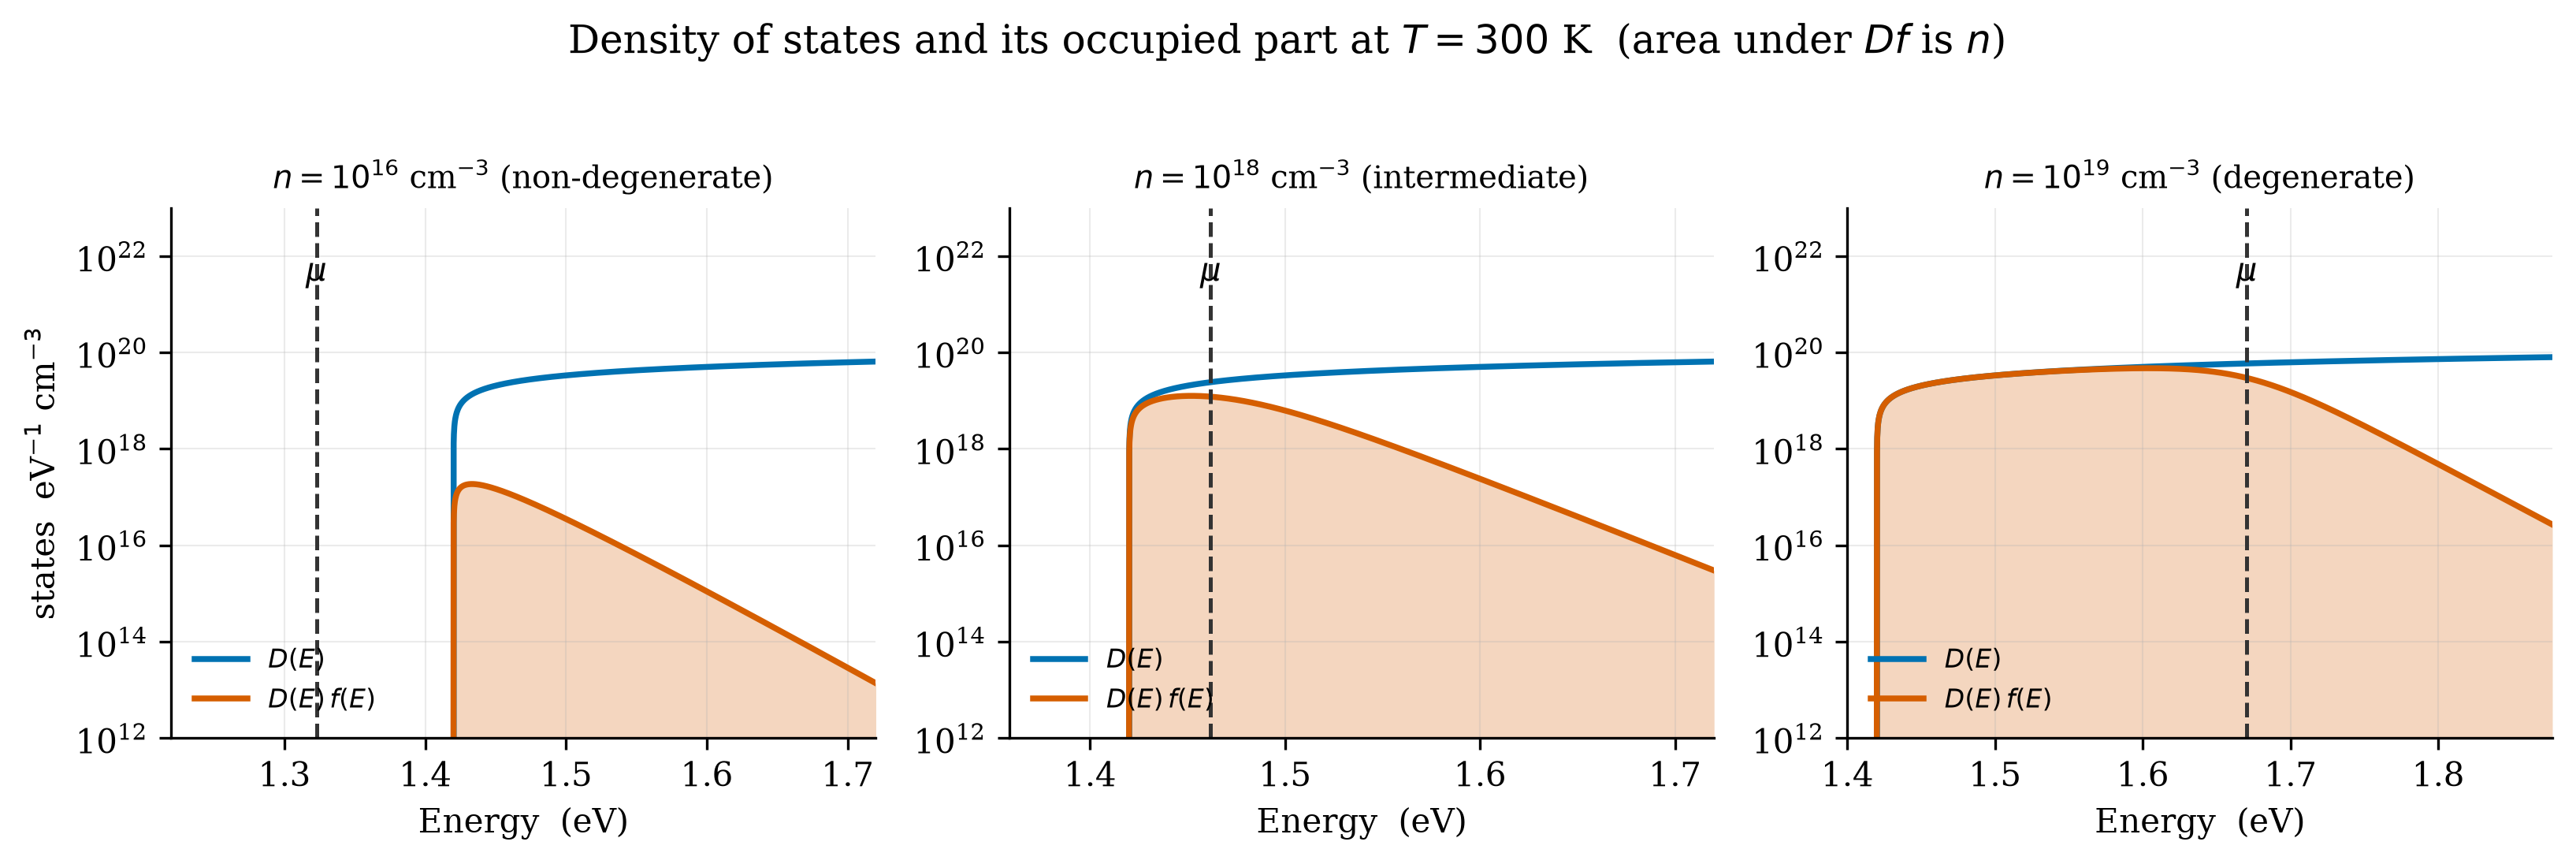
\includegraphics[width=\textwidth]{dos_occupied.png}
\caption{$D(E)$ and the occupied density of states $D(E)f(E)$ across the three regimes, at
$300$ K. A logarithmic axis is necessary: at $10^{16}\,$cm$^{-3}$ the occupied curve lies some
four orders of magnitude below $D(E)$ and would be indistinguishable from zero on a linear
scale. The area under $D(E)f(E)$ is $n$ in every panel. Both curves are the conduction-band
quantities only; the valence band and holes lie outside the model. The occupied curve is clipped
at $10^{10}\,$m$^{-3}$eV$^{-1}$ for plotting --- a floor on the axis, not on the physics, which
decays smoothly to zero.}
\label{fig:dos}
\end{figure*}

Figure~\ref{fig:dos} shows the same crossover in the occupation itself. In the non-degenerate
panel $D(E)f(E)$ falls exponentially above the band edge --- a straight line on the logarithmic
axis, the Boltzmann tail of Eq.~\eqref{eq:boltz}. In the degenerate panel it instead tracks
$D(E)$ itself right up to $\mu$ and then drops within a few $k_BT$: the states are simply filled
to the chemical potential, as they would be in a metal.

\subsection{Fermi level versus temperature}

\begin{figure*}[t]
\centering
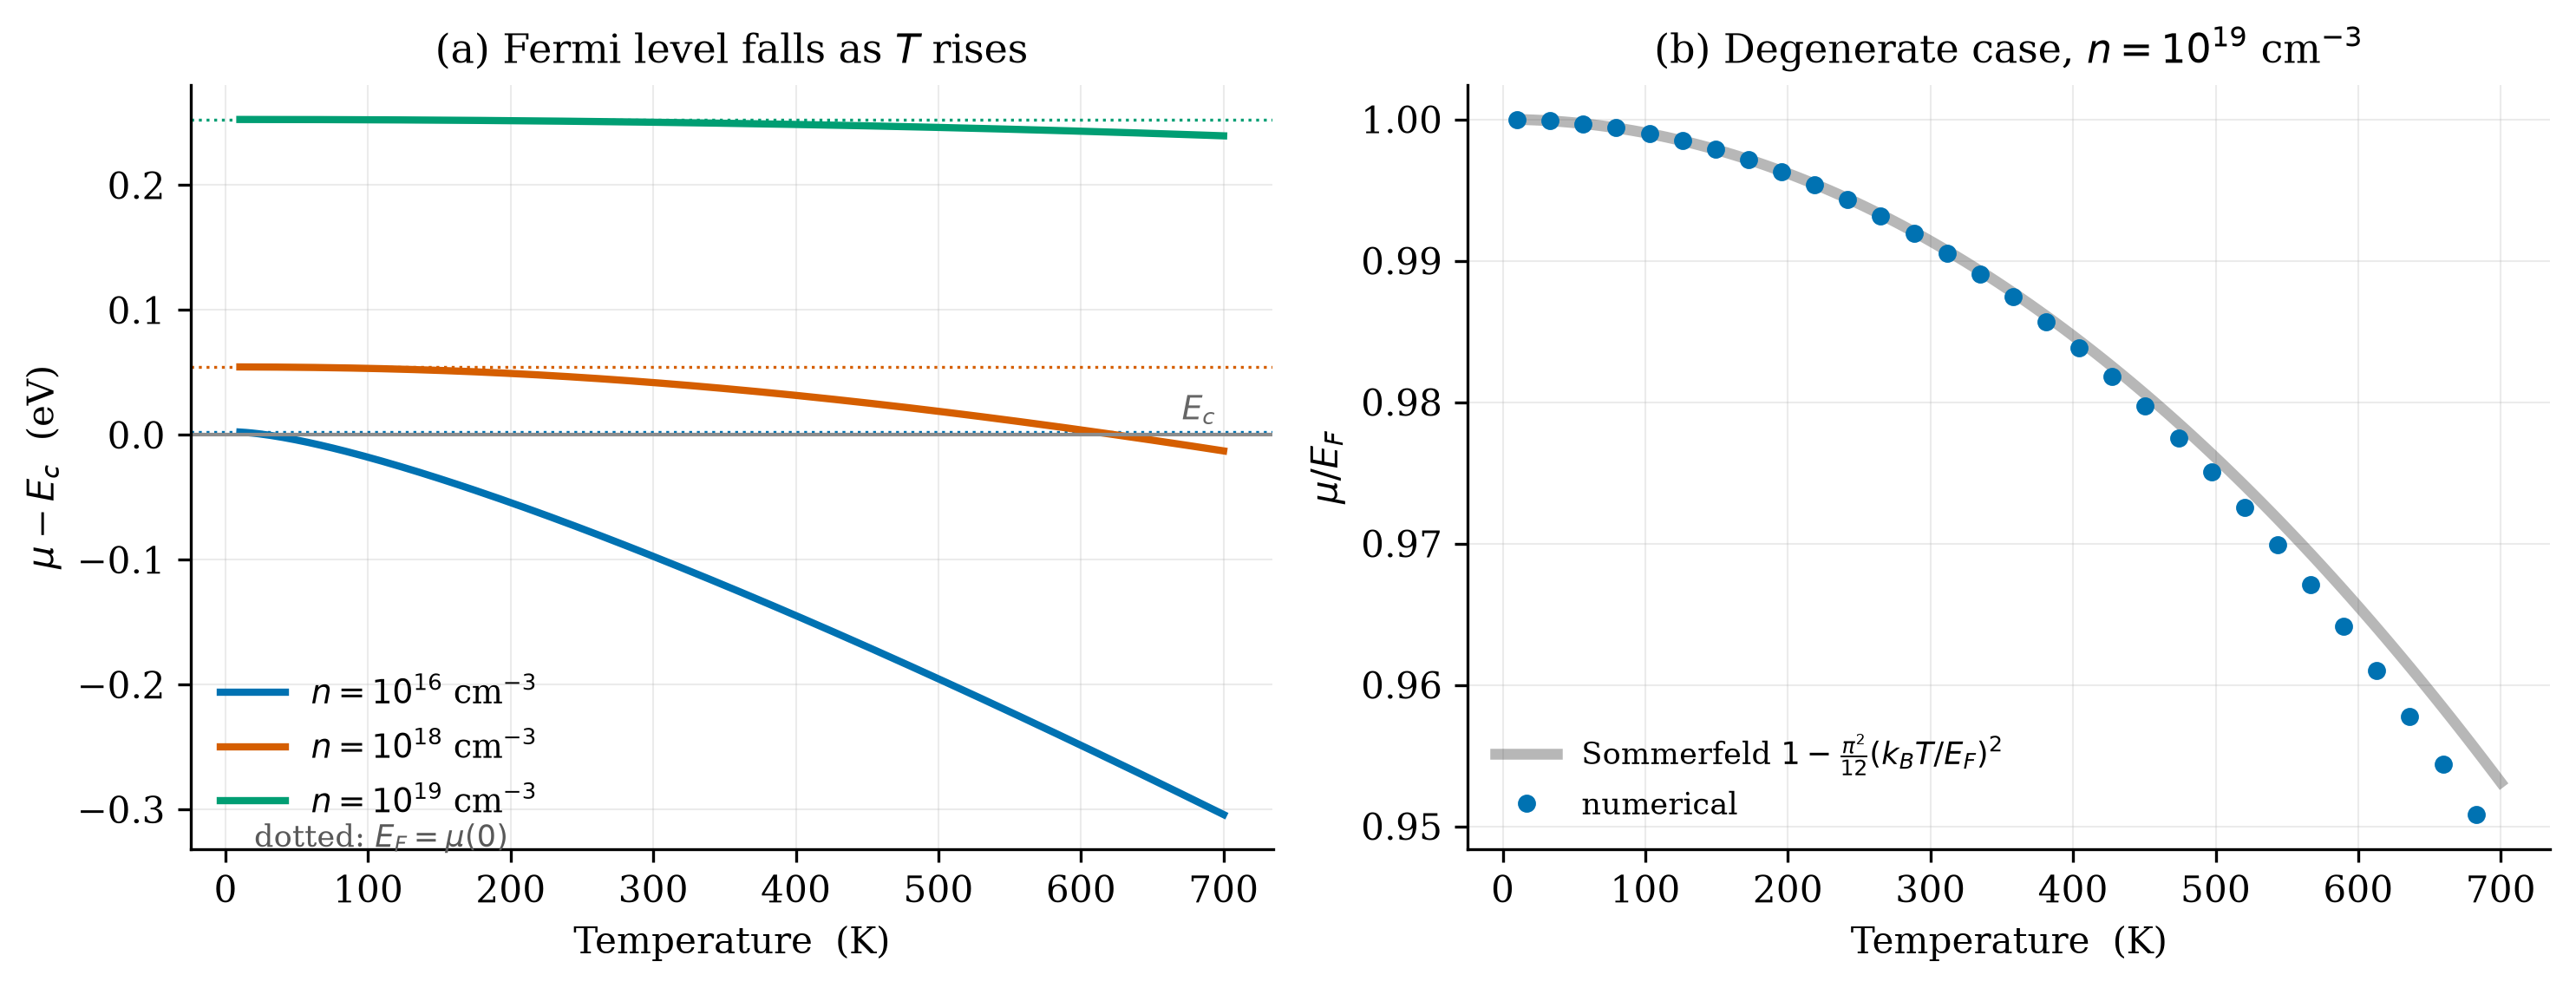
\includegraphics[width=\textwidth]{mu_vs_T.png}
\caption{(a) $\mu(T)$ at three carrier concentrations; dotted lines mark $E_F=\mu(0)$.
(b) The degenerate case at $10^{19}\,$cm$^{-3}$ against the Sommerfeld expansion
Eq.~\eqref{eq:somm}. The numerical points follow the analytic curve, departing from it by
$0.5\%$ only by $700$ K, where $k_BT/E_F$ is no longer small and the asymptotic expansion
begins to fail as expected.}
\label{fig:muT}
\end{figure*}

Figure~\ref{fig:muT}(a) shows $\mu$ falling as temperature rises, and the reason is the shape of
$D(E)$. The density of states grows as $\sqrt{E-E_c}$, so there are more states above $\mu$ than
below it within the thermal window. Raising $T$ promotes carriers upward into that larger
reservoir, and $\mu$ must fall to keep the total fixed. At low doping it falls below the band
edge entirely, which is the formal statement that the carriers have gone classical.

The degenerate case is far flatter, and Fig.~\ref{fig:muT}(b) shows why: the shift is the $T^2$
Sommerfeld correction of Eq.~\eqref{eq:somm}, which stays small while $k_BT \ll E_F$. The
numerical points follow the analytic curve closely up to about $300$ K and then begin to
separate, reaching a $0.5\%$ discrepancy at $700$ K where $k_BT/E_F \approx 0.24$. That
departure is the expected behaviour of an asymptotic expansion, and seeing where it begins is
more informative than a case chosen to hide it.

\subsection{Fermi level versus carrier concentration}

\begin{figure}[t]
\centering
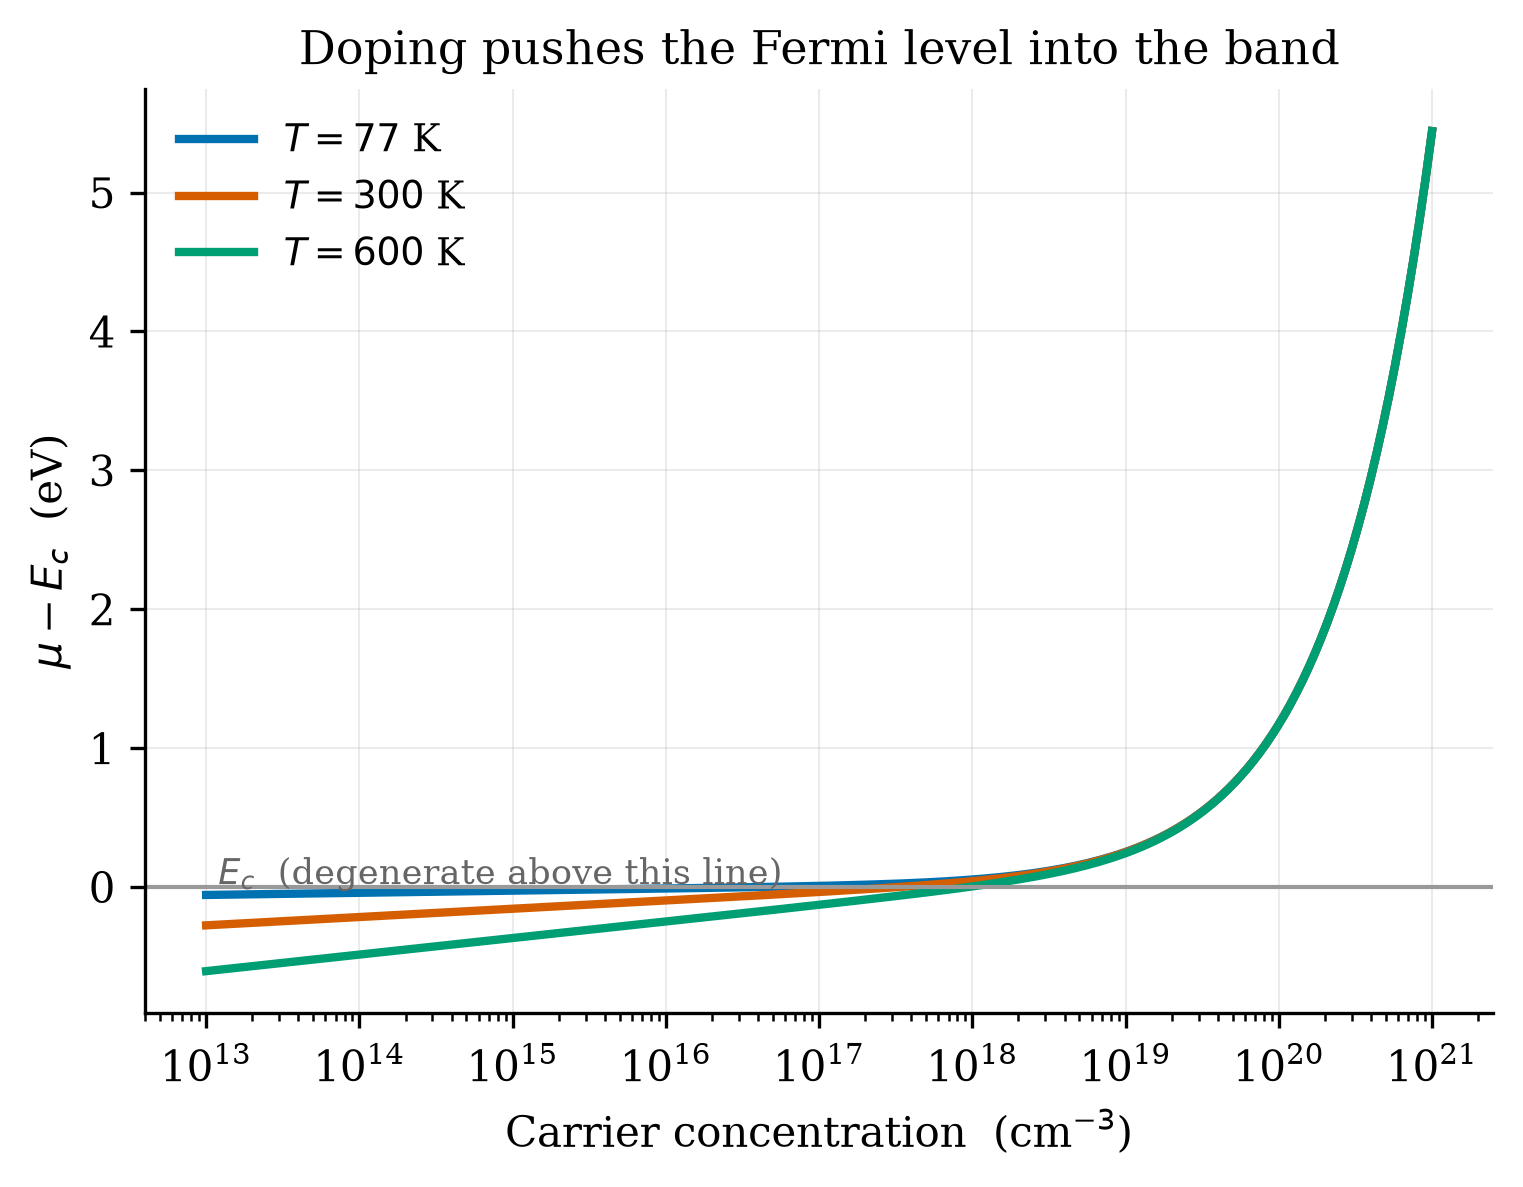
\includegraphics[width=\columnwidth]{mu_vs_n.png}
\caption{$\mu-E_c$ against carrier concentration at three temperatures. The curve crosses into
the band near $n \sim N_c$, which is $4.35\times10^{17}\,$cm$^{-3}$ for GaAs at $300$ K.}
\label{fig:mun}
\end{figure}

Figure~\ref{fig:mun} shows $\mu$ rising with doping, logarithmically at first and then more
steeply. The logarithmic stretch is Eq.~\eqref{eq:boltz} rearranged,
$\mu = E_c + k_BT\ln(n/N_c)$: in the non-degenerate regime the chemical potential depends only
on the \emph{ratio} $n/N_c$. The curve crosses $E_c$ near $n\simeq N_c$, and beyond that the
Pauli principle takes over --- further carriers must occupy higher states, and $\mu$ climbs as
$n^{2/3}$ from Eq.~\eqref{eq:EF}, far faster than logarithmically.

Raising the temperature shifts the crossing to higher $n$, because $N_c \propto T^{3/2}$: a hot
semiconductor has more thermally accessible states and needs heavier doping before degeneracy
sets in.

\subsection{Different materials}

\begin{table}[h]
\centering
\small
\begin{tabular}{lrrrr}
\toprule
Material & $E_g$ (eV) & $m^*/m_e$ & $\mu-E_c$ (meV) & $\eta$ \\
\midrule
GaAs & $1.42$ & $0.067$ & $-35.9$ & $-1.39$ \\
Si   & $1.12$ & $1.080$ & $-145.8$ & $-5.64$ \\
Ge   & $0.66$ & $0.560$ & $-120.3$ & $-4.65$ \\
\bottomrule
\end{tabular}
\caption{The three presets at $n=10^{17}\,$cm$^{-3}$ and $300$ K. The masses are
density-of-states masses, which already include the valley degeneracy (six $X$ valleys in
silicon, four $L$ in germanium), so $N_c$ must not be multiplied by it a second time. They are
larger than the conductivity masses quoted for mobility calculations.}
\label{tab:materials}
\end{table}

Table~\ref{tab:materials} isolates the role of the effective mass. All three materials carry the
same carrier concentration, yet GaAs is closest to degeneracy and silicon furthest from it. The
band gap is irrelevant to this --- it only sets where $E_c$ sits --- and the ordering follows
$m^*$ instead, through $N_c \propto (m^*)^{3/2}$. A light effective mass means few available
states, so a given carrier density fills them further up and pushes $\mu$ toward the band edge.
This is why GaAs, with the lightest electrons of the three, becomes degenerate at the lowest
doping.

\section{Conclusions}

Solving the carrier-density integral directly, rather than assuming either limit, gives a method
that spans the classical and degenerate regimes with one code path and reproduces both closed
forms where they apply --- to $1.3\times10^{-4}$ for the Boltzmann limit and $10^{-7}$ for the
degenerate limit. Applying it:

\begin{itemize}
  \item The classical--degenerate boundary sits near $n \sim N_c$, which for GaAs at $300$ K is
        $4.35\times10^{17}\,$cm$^{-3}$. Equivalently, degeneracy requires $T \ll T_F$.
  \item $\mu$ falls with temperature because $D(E)\propto\sqrt{E-E_c}$ offers more states above
        the chemical potential than below it; at low doping it drops below the band edge.
  \item In the degenerate regime that fall is the $T^2$ Sommerfeld correction, which the
        numerics reproduce until $k_BT/E_F$ ceases to be small.
  \item $\mu$ rises logarithmically with $n$ while non-degenerate and as $n^{2/3}$ once
        degenerate.
  \item Effective mass, not band gap, controls how readily a material becomes degenerate.
\end{itemize}

The model's limitations bound where it may be used. The band is a single isotropic parabolic
valley. Using density-of-states masses makes $N_c$ correct for the multi-valley materials, but
$k_F$ and $v_F$ computed from them describe one equivalent sphere rather than the real set of
anisotropic valleys. GaAs has $L$ and $X$ valleys only $0.29$ and $0.48$ eV above $\Gamma$, and
once $E_F$ approaches them those valleys hold carriers the model never counts --- the reason the
doping range above stops at $10^{19}\,$cm$^{-3}$. Band non-parabolicity
would reduce $E_F$ further at high doping. We also neglect the valence band and dopant
ionisation statistics, and treat $n$ as an input rather than solving for it self-consistently
from the dopant levels.

\section*{Reproducing this work}

\begin{verbatim}
uv venv --python 3.12 .venv
uv pip install -r requirements.txt
cd question_5
python test_fermi.py     # checks
python make_figures.py   # figures
streamlit run app.py     # interface
\end{verbatim}

\onecolumngrid
\appendix

\section{Complete source code}

Listings are included directly from the source files, so they cannot drift from the code that
produced the results above.

\subsection{\texttt{fermi.py} --- physics core}
\lstinputlisting{../fermi.py}

\subsection{\texttt{test\_fermi.py} --- validation suite}
\lstinputlisting{../test_fermi.py}

\subsection{\texttt{make\_figures.py} --- figure generation}
\lstinputlisting{../make_figures.py}

\subsection{\texttt{app.py} --- interactive interface}
\lstinputlisting{../app.py}

\twocolumngrid

\begin{thebibliography}{9}
\bibitem{kittel} C.~Kittel, \textit{Introduction to Solid State Physics}, 8th ed., Wiley, 2005.
  Chapter 6, the free-electron Fermi gas.
\bibitem{ashcroft} N.~W.~Ashcroft and N.~D.~Mermin, \textit{Solid State Physics},
  Holt--Saunders, 1976. Chapter 2 (Sommerfeld theory) and Chapter 28 (semiconductors).
\bibitem{sze} S.~M.~Sze and K.~K.~Ng, \textit{Physics of Semiconductor Devices}, 3rd ed.,
  Wiley, 2007. Chapter 1, carrier statistics.
\bibitem{blakemore} J.~S.~Blakemore, ``Approximations for Fermi--Dirac integrals'',
  \textit{Solid-State Electronics} \textbf{25}, 1067 (1982).
\bibitem{scipy} P.~Virtanen \textit{et al.}, ``SciPy 1.0: fundamental algorithms for scientific
  computing in Python'', \textit{Nature Methods} \textbf{17}, 261--272 (2020).
\bibitem{numpy} C.~R.~Harris \textit{et al.}, ``Array programming with NumPy'',
  \textit{Nature} \textbf{585}, 357--362 (2020).
\bibitem{streamlit} Streamlit documentation. \url{https://docs.streamlit.io}
\end{thebibliography}

\end{document}
